\section{Introduction}
\label{Section:SP}
 
Consider a point $\bfx$ from some $\cX \subseteq \BR^p$, and the spatial sign function $\bfS : \cX \times \BR^p \mapsto \BR^p$, defined as
%
$$
\bfS (\bfx; \bfmu_x) = \frac{\bfx - \bfmu_x}{\| \bfx - \bfmu_x \|}
\BI ( \bfx \ne \bfmu_x ),
$$
%
where $\bfmu_x \in \BR^p$ is a fixed location parameter, $\BI(\cdot)$ is the 0/1 indicator function and $\|.\|$ is the euclidean norm. This is a generalization of the real-valued case of the indicator for whether a point $x \in \BR$ is to the right, left or at a scalar $\mu_{x} \in \BR$, and was first introduced by \cite{MottonenOja95}. Given a data matrix $\bfX = (\bfx_{1}, \ldots, \bfx_{n})^T$, a popular approach of using spatial signs in the literature has been to take spatial signs of the data points, i.e. $\bfS(\bfx_i)$, and use the matrix of signs as a proxy of $\bfX$ to formulate robust versions of location and scale problems  \citep{locantore99, OjaBook10,WangPengLi15}.

The spatial sign maps all data points to the surface of a $p$-dimensional unit sphere (see Figure~\ref{fig:rankplot}). While this transformation has its advantages (i.e. robustness), e.g. the eigenvectors remain the same while limiting the influence of outliers when the points are drawn from an elliptical distribution \citep{taskinen12}, valuable information is lost in the form of magnitudes of sample points. As a result, spatial sign-based procedures suffer from low efficiency. For example, eigenvector estimates obtained from the covariance matrix of spatial sign, which is called the Sign Covariance Matrix (SCM), are asymptotically inadmissible \citep{magyar14}- in the sense that there is an estimator (namely, Tyler's M-estimate of scatter \citep{tyler87}) that has uniformly lower asymptotic risk than the SCM.

\paragraph{}
To utilize the magnitude information of sample points, at the same time preserving the robustness property, we propose a general class weighted spatial sign functions. To this end, we first propose what we call a {\it peripherality function}.

\begin{Definition}\label{defn:peripherality}
For a set of probability measures $\cM$ taking values in $\BR^p$, a {\it peripherality function} $ P : \BR^p \times \cM \mapsto \BR^+ \cup \{ 0\}$,  is a function that satisfies the following condition:\\

\noindent {\bf (P)} For every probability measure $\BF \in \cM$, there exists a constant $\bfmu_{F} \in \BR^p$ such that for any $t \in [ 0, 1]$ and $\bfx \in \BR^p$,
%
$$ 
P ( \bfmu_{F} ; \BF ) \leq P ( \bfmu_{F} + t ( \bfx - \bfmu_{F} ); \BF ). 
$$ 
%
That is, for every fixed $\BF$, the peripherality function achieves a minimum at $\mu_{F}$, and is non-decreasing in every direction away from $\bfmu_{F}$.
\end{Definition}

The peripherality function quantifies the relative position of $\bfx$ with respect to $\bfmu_{F}$, and condition (P) formalizes a general notion of centrality. A whole class of such functions can be defined from {\it Data Depth} functions \citep{zuo00}, which give the center-outward ranking of points in a multivariate dataset. Data depth has seen extensive use in the past decade, ranging from robust nonparametric classification \citep{jornsten04, ghosh05, dutta12, sguera14} to parametric estimation of means \citep{ZuoCuiHe04}, covariance matrices \citep{ZuoCui05} and sparse multivariate regression coefficients \citep{DuttaGenton17,MajumdarChatterjeeStat}. Peripherality functions can be defined as some inverse ranking based on data depth, and the concept of {\it outlyingness} associated with data depth is essentially same as what we use in this paper. However, traditional depth functions require a wider array of theoretical conditions \citep{zuo00} in addition to our condition (P), and a sizeable portion of methods we discuss do not require the use of depth functions {\it per se} to be implemented. %We use the term {\it peripherality} to keep track of the difference in application contexts and technical assumptions. As an additional objective of this paper, we discuss  some properties and uses of data-depth in real, separable Hilbert spaces.


%For t for which some mathematical 
%preliminaries are necessary for easier exposition. Let $(\Omega, \cA, \alpha)$ 
%be a probability space, and let $\cB$ be the Borel $\sigma$-algebra generated 
%by the norm topology of $\cH$. A $\cH$-valued random variable is a mapping 
%$X :  \Omega \rightarrow \cH$ such that for every $B \in \cB$, $X^{-1} (B) \in \cA$. 
%It is easy to see that $\alpha_{x} = \alpha ( X^{-1} (\cdot ) )$ is a probability 
%measure on the measurable space $(\cH, \cB)$. Mathematical details about 
%such probability measures on Hilbert spaces are available from a number of 
%places, including
%\bredbf
%BLSP notes (my primary reference), Gross, Segal, and what not.
%\eredbf
%
%
%Let $\cM$ be a set of probability measures on $\cH$. 
% If 
%we impose the practical restriction that $\inf_{x} P ( x ; F )$ is finite and 
%bounded below, then we may as well impose without loss of generality 
%$P ( \mu_{F} ; F ) = 0$ and consequently $P ( x ; F ) \geq 0$ for all $x \in \cH$ 
%and  $F \in \cM$. In many cases of interest, $P ( \cdot; \cdot)$ is 
%uniformly bounded above as well.
% 
%We will impose additional conditions on this function 
%as we proceed, but it can be seem immediately that any distance measure between 
%$x$ and $\mu_{F}$ satisfies the bare minimum requirement mentioned above. 

\begin{figure}[t]
	\captionsetup{singlelinecheck=off}
	\centering
		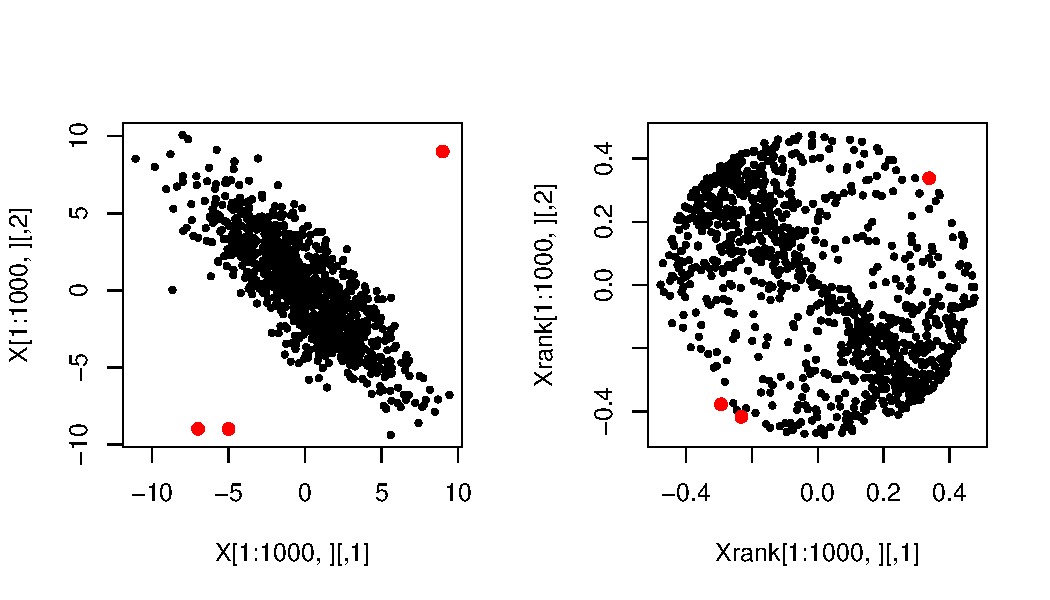
\includegraphics[height=6cm]{../Codes/ranks}
	\caption{(Left) 1000 points randomly drawn from $\mathcal N_2\left((0,0)^T, \left(\protect\begin{smallmatrix} 5 & -4 \\ -4 & 5 \protect\end{smallmatrix}\right)\right) $ and (Right) their signed peripherality functions based on halfspace depth}
	\label{fig:rankplot}
\end{figure}

Our weighted sign vector, which we call the {\it signed peripherality} function, is now defined as the product of the spatial sign and transformed peripherality functions:
%
\begin{align}\label{eqn:rank}
\bfR (\bfx; \bfmu_x, \BF) = \bfS(\bfx, \bfmu_x). \kappa_P( P(\bfx, \BF)),
\end{align}
%
where $\kappa_P: \BR \rightarrow \BR$ is a monotone function. Its purpose is to either downweight or upweight the spatial sign of a point based on its peripherality with respect to a data cloud. As seen in the third panel of Figure~\ref{fig:rankplot}, $\bfR (\bfx; \bfmu_x, \BF)$ maps points {\it inside} a ball of finite radius, thus limiting the influence of outlying points {\it and} preserving the magnitude information of data points. In this paper, we demonstrate certain interesting applications of this multivariate rank transformation in robust statistical inference. Notice that for the trivial choice $P( \bfx; \BF) = \| \bfx - \bfmu_{F} \|$ and $\bfmu_x = \bfmu_F, \kappa_P(x)=x$, we get $\bfR (\bfx; \bfmu_x, \BF) = \bfx$. However, in this paper we illustrate how using the rank-transformed data in place of the original data points or their spatial signs leads to interesting robustness results for other choices of the peripherality functions.

The notion of multivariate ranks goes back to \cite{PuriSenBook}, where they take the vector consisting of marginal univariate ranks as multivariate rank vector. Subsequent definitions of multivariate ranks were proposed by \cite{MottonenOja95,HallinPaindaveine02} and \cite{Chernozhukov14}. Compared to them, the advantages of our signed peripherality function are two-fold: interpretability and flexibility. Firstly, as evident in Figure~\ref{fig:rankplot}, our rank transformation preserves the general shape of the data. In fact, if the map $\| \bfx \| \rightarrow P(\bfx, \BF)$ is one-one (given a fixed $\BF$), then it is possible to get back $\bfx$ from $\bfR (\bfx; \bfmu_x, \BF)$. It also provides an intuitive extension to any spatial sign-based methodology. Secondly, there is considerable scope of generalization within the present framework. Given any general inner product space, the definition of signed peripherality remains the same when euclidean norm is replaced by the norm induced by the inner product. Even within $\BR^p$, it is possible to generalize the ranking function in \eqref{eqn:rank} by adding separate transformations on the sign and peripherality functions to obtain alternate representations of the data in lower or higher dimensional spaces. However, we limit our discussion in this paper to the original formulation in \eqref{eqn:rank}.

In this paper, we assume $\BF$ to be an elliptical distribution. Following \cite{FangEtal90}, elliptical distributions can be formally defined here using their characteristic function:
%
\begin{Definition}
A $p$-dimensional random vector $\bfX$ is said to elliptically distributed if and only if there exist a vector $\bfmu \in \mathbb R^p$, a positive semi-definite matrix $\Omega \equiv \Sigma^{-1} \in \mathbb R^{p \times p}$ and a function $\phi: \mathbb R_+ \rightarrow \mathbb R$ such that the characteristic function $\bft \mapsto \phi_{\bfX - \bfmu} (\bft)$ of $\bfX - \bfmu$ corresponds to $\bft \mapsto \phi (\bft^T \Sigma \bft), \bft \in \mathbb R^p$.
\end{Definition}
%
\noindent The density function of an elliptically distributed random variable takes the form:
%
$$
h(\bfx; \bfmu, \Sigma) = |\Omega|^{1/2} g ((\bfx - \bfmu)^T \Omega (\bfx - \bfmu)),
$$
%
where $g$ is a non-negative scalar-valued density function that is continuous and strictly increasing, and is called the \textit{density generator} of the elliptical distribution. For ease of notation, we denote such a distribution by $\mathcal{E} (\bfmu, \Sigma, g)$.


%{\it signed-peripherality function} $\kappa (\cdot)$. We define this function 
%with three parameters $\mu_{x} \in \cH$, $F \in \cM$ and  
%$\mu_{y} \in \cH$,  argument $x \in \cH$ and range $\cH$. More precisely,
%we use two functions $\kappa_{s} : \cH \rightarrow \cH$, 
%$\kappa_{p} : \cH \rightarrow \cH$ that are respectively 
%composed with the sign transformation and the peripherality function, and 
%then multiplied together to obtain the function
%$\kappa : \cH \times \cH \times \cM \times \cH \times \cH \rightarrow \cH$ 
%defined as 
%\ban 
%\kappa (x; \mu_{x}, F, \mu_{y} ) = k_{s} (S (x; \mu_{x})) k_{p} (P (x; F)) + \mu_{y}. 
%\ean
%Within this very generic framework, we will explore two simple choices. We consider 
%$\kappa_{s} (x) = x$, thus this is fixed to be the identity transformation. The two 
%alternatives we consider for $\kappa_{p}$ are 
%$\kappa_{p} (x) = x$ and $\kappa_{p} (x) = \exp (- x)$, thus one is linearly 
%increasing with $x$ while the other is exponentially decreasing.
%
%
%Notice that if we consider $\mu_{y} = \mu_{F} = \mu_{x}$,  
%$\kappa_{s} (x) = \kappa_{p} (x) = x$, and take the very 
%simple peripherality  function $P( x; F) = || x - \mu_{F} ||$, we have 
%$\kappa (x; \mu_{x}, F, \mu_{y} ) \equiv x$ for all choices of parameters 
%$\mu_{x}, F, \mu_{y}$.  Consequently, under this choice of parameters for the 
%$\kappa$-transformation, analyzing a dataset $\{ X_{1}, \ldots, X_{n} \}$ and 
%its $\kappa$-transformed version 
%$\{ Y_{i} = \kappa (X_{i}; \ldots), \ i = 1, \ldots, n \}$ are equivalent. However,
%in this paper we illustrate how other choices of the peripherality function 
%lead to interesting robustness results. We have deliberately set the location 
%parameters $\mu_{x}, \mu_{F}, \mu_{y}$ to be potentially non-identical, this 
%additional flexibility has some advantage for robust data analysis. In many 
%applications, the value of these three parameters may be identical, which leads 
%to no conflict in our framework.

\paragraph{Organization of paper.}

\paragraph{Notation.}
